\documentclass[twocolumn, 10pt, a4j]{jsarticle}
  \usepackage{here}
  \usepackage{amsmath}
  \usepackage[dvipdfmx]{graphicx}
  \usepackage{url}
  % プリアンブル
  \title{\vspace{-2.5cm}振動の計測と制御}
  \author{1610581 堀田 大地}
  \date{2018/7/26}
  \begin{document}
  \maketitle{}
  \section{結果}
    結果を表1に示した. また,加速度センサの各周波数における出力波形を図1,2,3,4,5に示した.周波数が大きくなるごとに波の周期が短くなっていった.
      % 表1
    \begin{table}[]
      \centering
        \caption{周波数Hzと$dx mS, dy V$の関係}
        \label{my-label}
        \footnotesize
        \begin{tabular}{lll}
          周波数Hz V & $dx$ mV& $dy V$ \\ \hline
          20 & 27.039 & -14.744 \\
          40 & 12.085 & -35.329 \\
          60 & 7.935 & -24.329 \\
          80 & 6.104 & -21.630 \\
          100 & 4.700 & -19.188 \\
        \end{tabular}
      \end{table}

      \begin{figure}[H]
        % 図1
        \begin{center}
          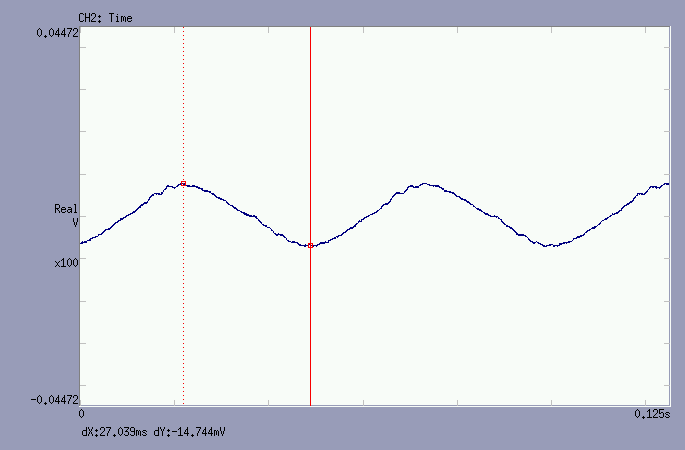
\includegraphics[width=7cm]{../img/experiments/001.png}
          \caption{周波数20Hz}
        \end{center}
      \end{figure}

      \begin{figure}[H]
        % 図2
        \begin{center}
          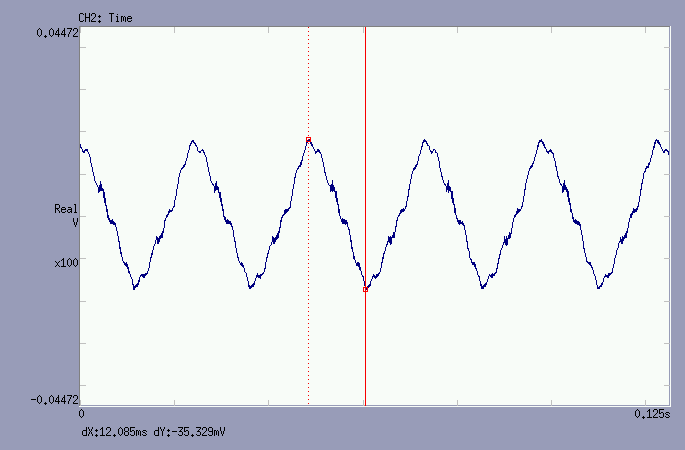
\includegraphics[width=7cm]{../img/experiments/002.png}
          \caption{周波数40Hz}
        \end{center}
      \end{figure}

      \begin{figure}[H]
        % 図3
        \begin{center}
          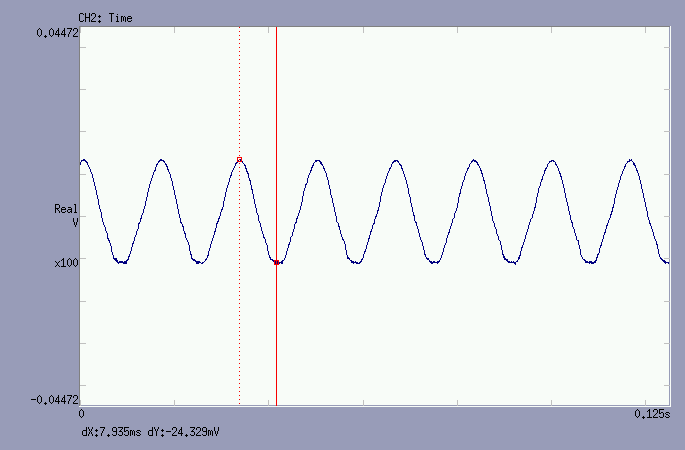
\includegraphics[width=7cm]{../img/experiments/003.png}
          \caption{周波数60Hz}
        \end{center}
      \end{figure}
      \begin{figure}[H]
        % 図4
        \begin{center}
          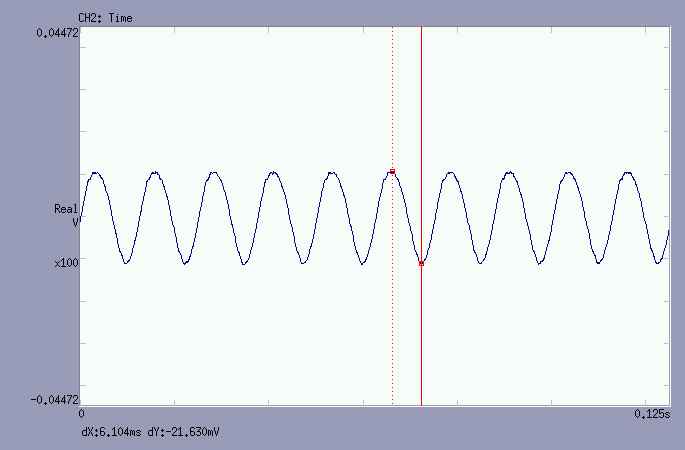
\includegraphics[width=7cm]{../img/experiments/004.png}
          \caption{周波数80Hz}
        \end{center}
      \end{figure}
      \begin{figure}[H]
        % 図5
        \begin{center}
          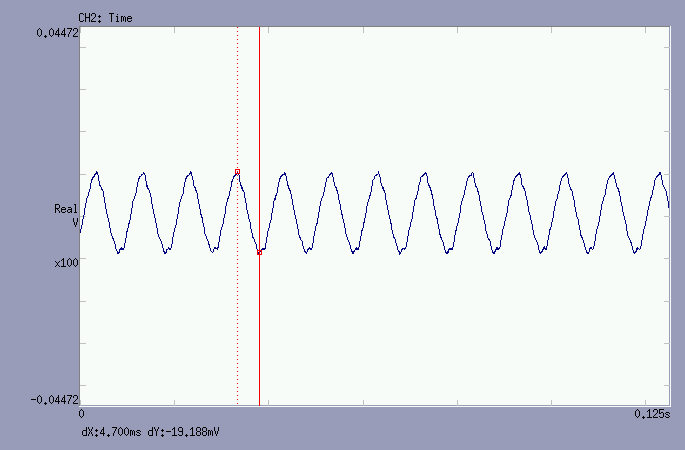
\includegraphics[width=7cm]{../img/experiments/005.png}
          \caption{周波数100Hz}
        \end{center}
      \end{figure}

  \end{document}